\section{Results}\label{results}

\subsection{Run integrity and panel scale}

The full diagnostic-reference panel completed 144 annual EnergyPlus selection-role cases, representing 119 unique source-year weather trajectories. Each trace contains 35{,}040 records and 16{,}704 occupied records, yielding 2{,}405{,}376 occupied records in the prespecified role-weighted panel. The trace schema was consistent across cases, all 45 raw zone environmental fields were populated during occupied periods, and no fatal EnergyPlus errors occurred. Sixteen cases reported warmup-convergence Severe messages, but EnergyPlus completed successfully in each case. These messages are treated as simulation QA limitations rather than failed cases. The synchronized post-processing audit completed all 144 role cases, verified the 119 unique state arrays, and reproduced identical outputs for duplicate roles that referenced the same environmental state.

Because the diagnostic-reference strategy did not use the probability outputs to adjust setpoints, the results below describe representation behavior under fixed simulated environments. They should not be read as closed-loop HVAC outcomes.

\subsection{Mean TSV and TSV-tail probability}

Across the full role-weighted panel, mean $p_{\mathrm{tail}}$ was 0.116 and the 95th percentile was 0.304. Using the screening cutoff $p_{\mathrm{tail}}\ge0.20$, 13.15\% of occupied records were high-tail states. Exceedance was similar in the reference 2025--2029 and near-2030s slices (8.91\% and 8.89\%), then increased in the mid-2050s and late-2080s slices (13.96\% and 20.84\%; Table~\ref{tab:panel_tail_summary}). The typical-year selector showed the same ordering, with 6.93\%, 7.23\%, 10.06\%, and 16.60\% high-tail exceedance across the four slices. SSP2-4.5 had 11.45\% high-tail exceedance, while SSP5-8.5 had 14.85\%. Giving each of the 119 unique environmental states equal weight changed mean-zone high-tail exceedance from 13.15\% to 12.44\%, any-zone exceedance from 36.64\% to 35.41\%, and hidden any-zone exceedance from 23.50\% to 22.98\%; the aggregation pattern was unchanged (Supplementary Table~S1).

\begin{table}[htbp]
\centering
\caption{High-tail exceedance summary for the 144-case, selection-role-weighted fixed-reference panel. High-tail exceedance is the share of occupied records with $p_{\mathrm{tail}}\ge0.20$.}
\label{tab:panel_tail_summary}
\footnotesize
\begin{tabular}{llrr}
\toprule
\textbf{Grouping} & \textbf{Level} & \textbf{Mean $p_{\mathrm{tail}}$} & \textbf{High-tail exceedance (\%)} \\
\midrule
All & Full panel & 0.116 & 13.15 \\
\midrule
Scenario & SSP2-4.5 & 0.111 & 11.45 \\
Scenario & SSP5-8.5 & 0.120 & 14.85 \\
\midrule
Time slice & baseline\_2020s & 0.104 & 8.91 \\
Time slice & near\_2030s & 0.104 & 8.89 \\
Time slice & mid\_2050s & 0.117 & 13.96 \\
Time slice & late\_2080s & 0.136 & 20.84 \\
\midrule
Severity & typical & 0.108 & 10.21 \\
Severity & hot & 0.119 & 14.48 \\
Severity & heatwave\_extreme & 0.120 & 14.76 \\
\bottomrule
\end{tabular}
\end{table}

City differences were large. Kolkata had the highest mean-zone high-tail exceedance (19.53\%), followed by Ahmedabad (16.65\%), Phoenix (13.02\%), Guangzhou (12.22\%), Houston (12.09\%), and Beijing (5.37\%). The highest case-level exceedance rates occurred in hot or heatwave-extreme late-century files. In Kolkata under SSP5-8.5 in the late-2080s, the hot and heatwave-extreme selectors coincided on one source year, which had 40.65\% high-tail exceedance.

A paired block bootstrap that resampled the 48 city--scenario--time-slice blocks gave a mean-zone screened share of 13.15\% [11.02, 15.45], an any-zone share of 36.64\% [32.39, 40.87], and a mean-hidden any-zone gap of 23.50 percentage points [20.79, 26.12]. Relative to the reference slice, the near-2030s contrast was $-0.02$ percentage points [$-2.00$, 1.70], the mid-2050s contrast was $+5.05$ [1.81, 9.03], and the late-2080s contrast was $+11.93$ [8.10, 16.31]. These intervals quantify sensitivity to the finite case panel; they are not population or climate-model uncertainty intervals.

\begin{figure}[H]
    \centering
    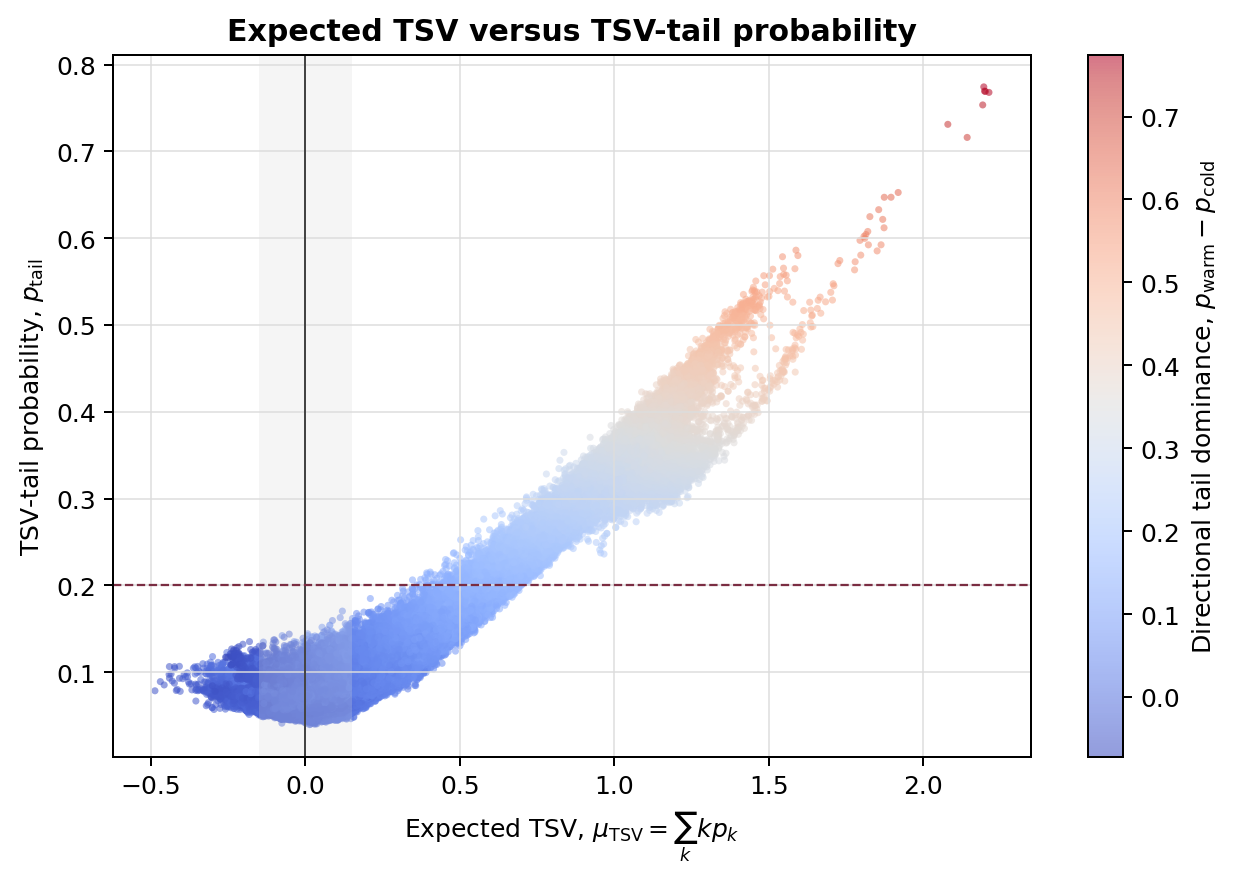
\includegraphics[width=0.86\linewidth]{figs/mean_vs_tail_scatter_sample.png}
    \caption{Expected TSV versus TSV-tail probability for a sampled subset of the 144-case diagnostic panel. Expected TSV denotes the probability-weighted mean $\mu_{\mathrm{TSV}}=\sum_k k p_k$, not the most likely TSV class. The horizontal line marks the illustrative reporting screen $p_{\mathrm{tail}}=0.20$. Expected TSV is informative, but $p_{\mathrm{tail}}$ directly reports the modeled probability mass in the selected TSV categories.}
    \label{fig:mean_tail_scatter}
\end{figure}

Figure~\ref{fig:mean_tail_scatter} shows the internal relationship between the TSV probability distribution and two summaries derived from it. Expected TSV remained strongly associated with TSV-tail probability, so the scalar mean is not meaningless. The diagnostic does not show near-neutral high-tail states under the strict condition $|\mu_{\mathrm{TSV}}|<0.15$; that share was 0.0\%. The stronger finding is different: similar positive mean states can still carry different tail probabilities. Within 0.05-wide expected-TSV bins, the 5th--95th percentile spread in $p_{\mathrm{tail}}$ reached 0.145 in the populated $\mu_{\mathrm{TSV}}=1.35$--1.40 bin ($n=1{,}204$). A scalar mean gives the warm-side tendency, but the probability distribution shows how much mass is assigned to the warm/hot outer categories.

The same figure also shows that TSV-tail probability in this fixed-reference panel is warm-dominant. Mean warm-tail probability was 0.088, compared with 0.027 for the cold tail. Warm-tail probability exceeded cold-tail probability in 78.3\% of occupied records and in all records crossing $p_{\mathrm{tail}}\ge0.20$. Records with $\mu_{\mathrm{TSV}}\le0$ never crossed the high-tail screen, while all records with $\mu_{\mathrm{TSV}}>1$ did. Thus, above about $+1$ expected TSV, the scalar mean already identifies a warm-tail state; the probability distribution is still needed to quantify the associated outer-category mass.

\subsection{PMV as a scalar benchmark}

The PMV comparison gives a second scalar benchmark. Across the same occupied records, $|\mathrm{PMV}|$ was correlated with $p_{\mathrm{tail}}$ (Pearson $r=0.859$, Spearman $\rho=0.752$), while $|\mu_{\mathrm{TSV}}|$ was more tightly correlated with $p_{\mathrm{tail}}$ (Pearson $r=0.975$, Spearman $\rho=0.895$). A best offline $|\mu_{\mathrm{TSV}}|$ threshold of 0.608 disagreed with the high-tail flag in 1.07\% of occupied records. A best offline $|\mathrm{PMV}|$ threshold of 0.913 disagreed in 3.27\% of occupied records.

\begin{figure}[H]
    \centering
    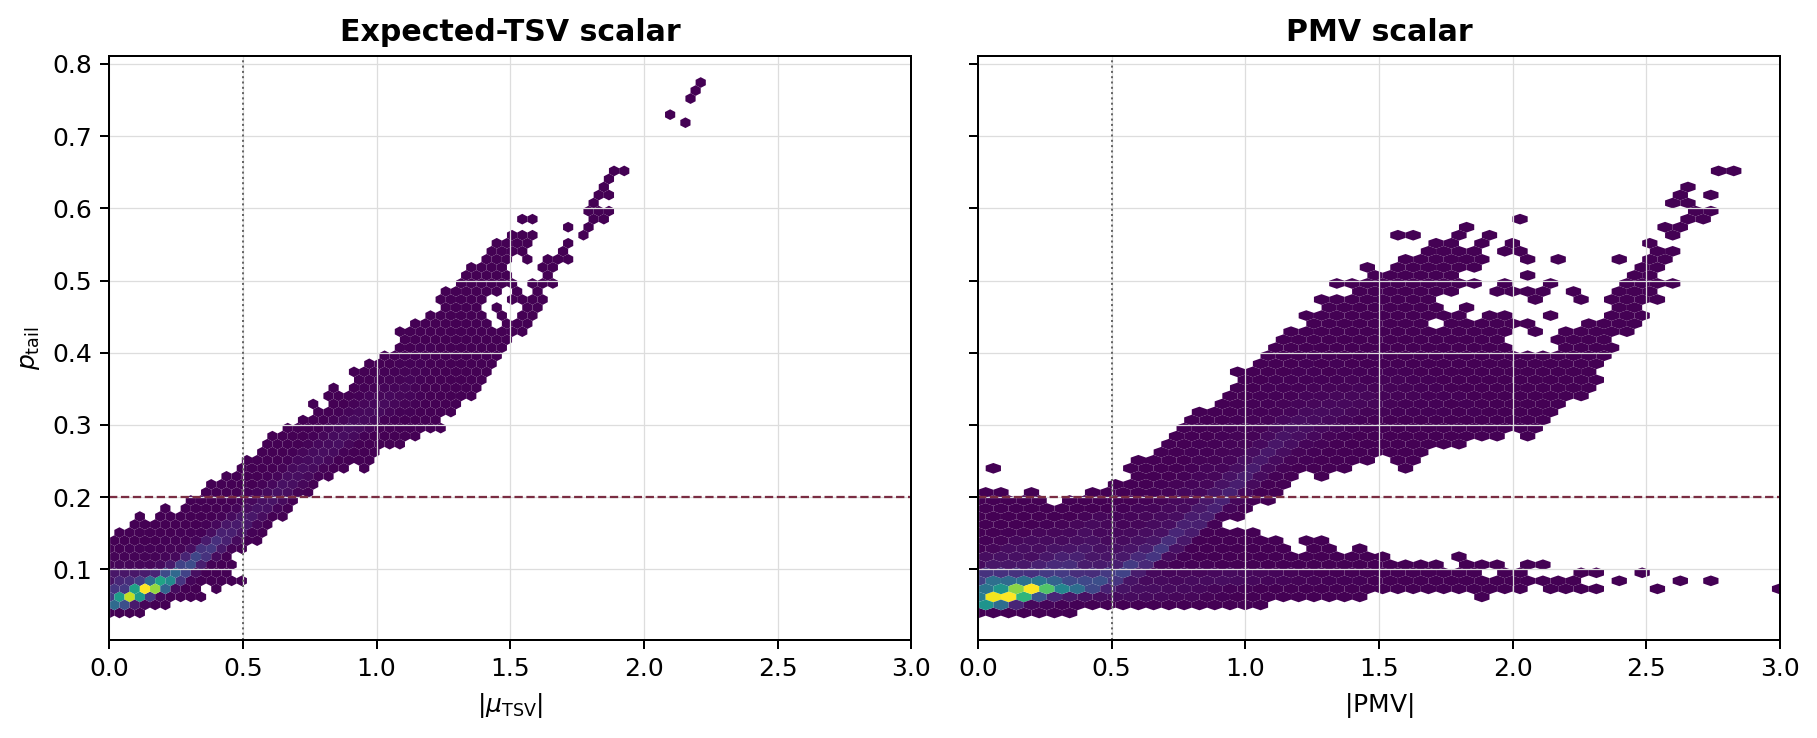
\includegraphics[width=\linewidth]{figs/scalar_tail_comparison_hexbin.png}
    \caption{Scalar comparison against the primary TSV probability output. Left: $|\mu_{\mathrm{TSV}}|$ versus $p_{\mathrm{tail}}$. Right: $|\mathrm{PMV}|$ versus the same $p_{\mathrm{tail}}$ distribution. Both panels use the same 0--3 scalar range. The vertical line marks the conventional 0.5 scalar band, and the horizontal line marks the diagnostic high-tail screen $p_{\mathrm{tail}}=0.20$.}
    \label{fig:pmv_scalar_comparison}
\end{figure}

\begin{table}[htbp]
\centering
\caption{Scalar threshold comparison against the $p_{\mathrm{tail}}\ge0.20$ high-tail flag. Best thresholds are optimized offline over the full diagnostic panel. Missed high-tail and false-positive rates are reported as percentages of all occupied records.}
\label{tab:pmv_scalar_comparison}
\scriptsize
\resizebox{\textwidth}{!}{%
\begin{tabular}{lrrrr}
\toprule
\textbf{Scalar rule} & \textbf{Threshold} & \textbf{Disagreement (\%)} & \textbf{Missed high-tail (\% records)} & \textbf{False positive (\% records)} \\
\midrule
$|\mu_{\mathrm{TSV}}|$ best threshold & 0.608 & 1.07 & 0.61 & 0.46 \\
$|\mathrm{PMV}|$ best threshold & 0.913 & 3.27 & 1.50 & 1.76 \\
$|\mathrm{PMV}|$ standard band & 0.500 & 18.93 & 0.003 & 18.92 \\
\bottomrule
\end{tabular}
}
\end{table}

Read together, Figures~\ref{fig:mean_tail_scatter} and~\ref{fig:pmv_scalar_comparison} separate two issues. Figure~\ref{fig:mean_tail_scatter} shows how the learned TSV expectation relates to its own tail probability. Figure~\ref{fig:pmv_scalar_comparison} asks how that relationship differs from PMV, Fanger's continuous comfort index built from thermal-balance terms and empirical chamber-vote evidence. The standard $|\mathrm{PMV}|=0.5$ band behaved conservatively in this panel. It almost never missed high-tail states, but it flagged many states that did not cross $p_{\mathrm{tail}}\ge0.20$. The learned expected-TSV scalar occupies a narrower range and follows the calibrated tail probability closely because both are summaries of the same seven-class probability vector. This is a tighter empirical association, not a claim of linearity: $|\mu_{\mathrm{TSV}}|$ reports the location of the predicted distribution, while $p_{\mathrm{tail}}$ reports its outer-category mass. Its maximum absolute value was 2.24 in this panel, and only 3.5\% of occupied records exceeded $|\mu_{\mathrm{TSV}}|=1$. PMV spans a wider scalar range, reaching 3.31 in absolute value, and includes a lower-$p_{\mathrm{tail}}$ branch at higher $|\mathrm{PMV}|$ values. This broad branch around $p_{\mathrm{tail}}\approx0.1$ is the visual source of the conservative PMV result: PMV can assign a large scalar departure to states that the calibrated TSV distribution still places mostly in neutral or mild categories. Among records with $|\mathrm{PMV}|\ge0.5$, 59.0\% remained below $p_{\mathrm{tail}}=0.20$; even among records with $|\mathrm{PMV}|\ge1$, 9.3\% remained below that tail-probability screen. The mid-tail band shows the same compression: for records with $0.3\le p_{\mathrm{tail}}<0.4$, the 5th--95th percentile range was 0.88--1.20 for $|\mu_{\mathrm{TSV}}|$ but 1.05--1.86 for $|\mathrm{PMV}|$. The point is not that PMV is useless or blind to thermal stress; rather, PMV and $p_{\mathrm{tail}}$ answer different diagnostic questions. PMV gives a conventional continuous mean-vote index for the thermal state. $p_{\mathrm{tail}}$ reports the predicted probability mass in the selected TSV categories.

The no-PMV robustness check gave the same qualitative result, but it should be read as a model-output comparison rather than as two versions of PMV. Figure~\ref{fig:pmv_feature_robustness} keeps the x-axis fixed as the same synchronized $|\mathrm{PMV}|$ scalar and changes the y-axis from the primary $p_{\mathrm{tail}}$ output to the $p_{\mathrm{tail}}$ output from a separately trained no-PMV TSV predictor. Removing PMV from the ordinal predictor changed the mean-zone high-tail exceedance at $p_{\mathrm{tail}}\ge0.20$ from 13.15\% to 13.85\%, and changed any-zone exceedance from 36.64\% to 37.52\%. The PMV-inclusive output is modestly tighter against the PMV scalar, with Pearson $r=0.859$ and Spearman $\rho=0.752$, compared with $r=0.857$ and $\rho=0.738$ for the no-PMV output. This supports a limited interpretation: calculable PMV is a useful predictor feature for reported TSV probabilities, but the main scalar-reference and aggregation results are not created solely by including PMV in the model. Under the no-PMV predictor, $|\mu_{\mathrm{TSV}}|$ still had Pearson $r=0.976$ with its own $p_{\mathrm{tail}}$ output. We therefore treat the PMV comparison as a descriptive scalar-reference audit, not as the main evidence for the probability diagnostic.

The saved nominal seven-class predictor provides a separate model-form check on the ordinal representation. At $p_{\mathrm{tail}}\ge0.20$, the nominal model's mean-zone, area-weighted mean-probability, p90-zone, and any-zone screened shares were 14.34\%, 12.74\%, 27.86\%, and 35.16\%, respectively, compared with 13.15\%, 12.13\%, 27.83\%, and 36.64\% for the ordinal model. The largest absolute rate difference was 1.48 percentage points, and both models preserved the ordering between mean, p90, and any-zone screens across the prespecified threshold range. The spatial conclusion is therefore a property of retaining categorical probabilities in this application, not an observed advantage that appears only under the cumulative ordinal algorithm.

\begin{figure}[htbp]
    \centering
    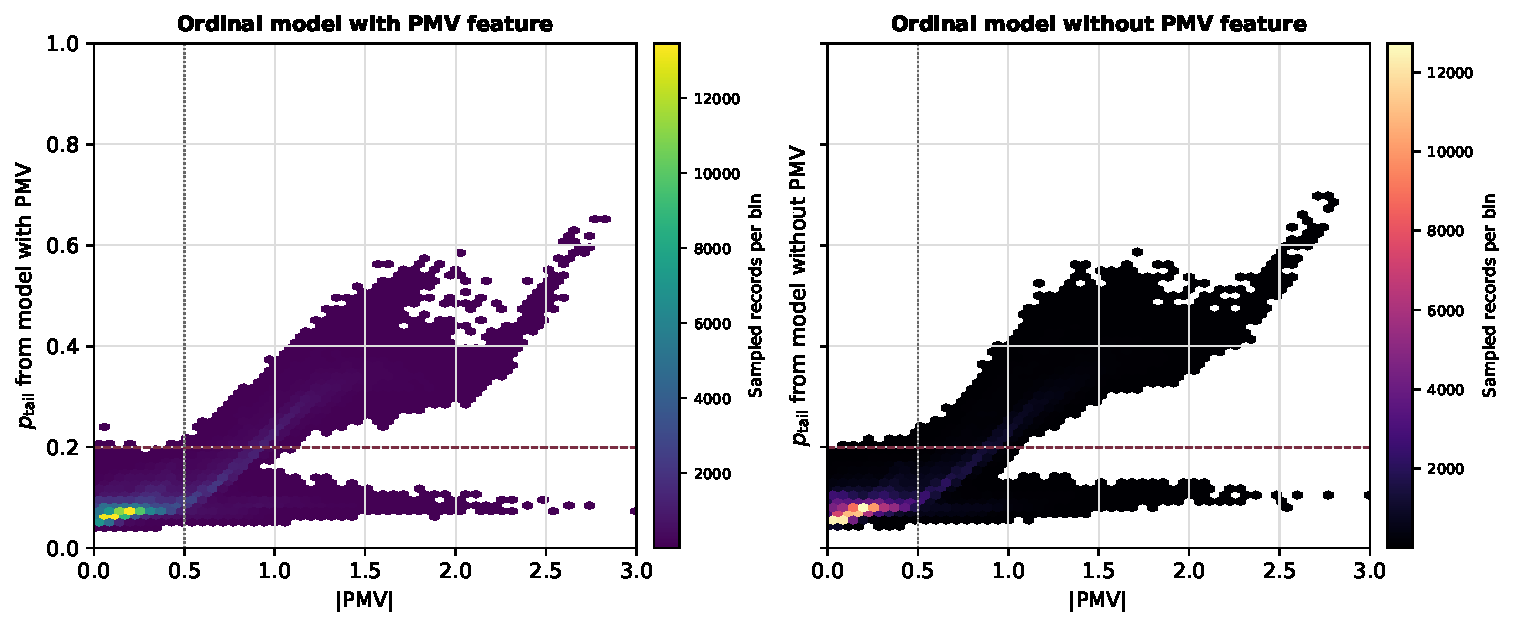
\includegraphics[width=\linewidth]{figs/pmv_feature_robustness_hexbin.pdf}
    \caption{PMV-scalar robustness check using two TSV probability outputs. Both panels use the same x-axis scalar, $|\mathrm{PMV}|$, from the simulated thermal state. The left panel plots PMV against $p_{\mathrm{tail}}$ from the primary TSV predictor, which includes PMV as an engineered covariate. The right panel plots the same PMV values against $p_{\mathrm{tail}}$ from a separately trained no-PMV TSV predictor. The different palettes indicate that the two panels contain different probability-model outputs, not different PMV calculations.}
    \label{fig:pmv_feature_robustness}
\end{figure}

For the probability metrics below, the Brier score is mean squared error of the binary tail probability; fixed-bin expected calibration error (ECE) is the bin-count-weighted absolute predicted--observed gap; area under the receiver operating characteristic curve (AUROC) and average precision summarize ranking discrimination; and F1 is the harmonic mean of precision and recall at the stated $p_{\mathrm{tail}}\ge0.20$ screen.

The pooled held-out TSV validation check gives the same practical reading (Tables~\ref{tab:tail_probability_comparison} and~\ref{tab:tsv_predictor_validation}). The primary and no-PMV predictors had nearly identical point performance: exact-class accuracy was 47.3\% and 46.9\%, within-one-class accuracy was 84.1\% and 83.8\%, and ordinal class MAE was 0.73 for both. The rounded-PMV class baseline was weaker on exact and ordinal metrics, with 33.2\% exact accuracy and 0.97 class MAE. Class-specific recall was modest in the tail classes for all methods, consistent with the neutral-heavy and noisy structure of field TSV data. Supplementary calibration checks show that aggregate predicted $p_{\mathrm{tail}}$ aligned closely with observed tail frequency on the held-out split: the primary model's mean predicted $p_{\mathrm{tail}}$ was 0.207 versus an observed tail frequency of 0.206, with fixed-bin tail ECE of 0.011. We also tested a PMV-only calibrated tail baseline, fitted as $|\mathrm{PMV}|\rightarrow\Pr(\mathrm{TSV}\le-2\ \mathrm{or}\ \mathrm{TSV}\ge+2)$ on the same non-test data. Table~\ref{tab:tail_probability_comparison} shows that this baseline matched overall tail prevalence but discriminated tail records less well than the TSV probability models. AUROC was 0.571 versus 0.747, average precision was 0.260 versus 0.483--0.487, Brier score was 0.161 versus 0.137--0.138, and F1 at the $p_{\mathrm{tail}}\ge0.20$ screen was 32.6\% versus 46.4--47.1\%. Contributor-clustered paired intervals preserved the primary model's advantage over the PMV-only baseline in Brier score, AUROC, and average precision, whereas every primary-versus-no-PMV interval included zero. A stricter contributor-grouped robustness check gave 42.1\% exact accuracy, 79.8\% within-one-class accuracy, tail AUROC of 0.577, and F1 of 32.5\%. This weaker transfer limits any absolute reading of simulated TSV-tail percentages under domain shift. The supported claim is therefore limited: primary and no-PMV held-out performance is similar, PMV alone contains useful but less discriminative tail information, and the diagnostic should not be treated as a PMV-only artifact.

An overlap-excluded reciprocal source-label holdout provided a separate domain-shift check. Six city--year strata with likely cross-source study overlap were removed from both corpora before refitting. Tail AUROC was 0.592 for ASHRAE-to-China and 0.553 in the reverse direction; tail ECE was 0.096 and 0.124, while mean predicted versus observed tail prevalence shifted from 0.225 versus 0.165 to 0.121 versus 0.223. Class-distance metrics did not consistently improve on an always-neutral target baseline. Transport therefore degraded materially across the two source labels. This check evaluates the fitting pipeline under source shift; the final pooled predictor has not been evaluated on a wholly unused third corpus.

\begin{table}[htbp]
\centering
\caption{Held-out tail-probability comparison for the TSV probability models and the PMV-only calibrated scalar baseline. F1 is computed by screening each predicted tail probability at $p_{\mathrm{tail}}\ge0.20$.}
\label{tab:tail_probability_comparison}
\scriptsize
\setlength{\tabcolsep}{4.2pt}
\begin{tabular}{lrrrrrr}
\toprule
\textbf{Predictor} & \textbf{Mean predicted} & \textbf{Observed} & \textbf{Brier} & \textbf{ECE} & \textbf{F1 (\%)} & \textbf{AUROC} \\
\midrule
Primary TSV model & 0.207 & 0.206 & 0.137 & 0.011 & 47.1 & 0.747 \\
No-PMV TSV model & 0.207 & 0.206 & 0.138 & 0.006 & 46.4 & 0.747 \\
PMV-only calibrated tail baseline & 0.206 & 0.206 & 0.161 & 0.003 & 32.6 & 0.571 \\
\bottomrule
\end{tabular}
\end{table}

\begin{table}[htbp]
\centering
\caption{Held-out TSV class validation for the primary predictor, the no-PMV robustness predictor, and a rounded-PMV class baseline. The PMV baseline rounds PMV to the nearest TSV class and clips to $[-3,+3]$; it is a deterministic scalar-label baseline, not a probability model. Argmax-tail F1 converts each probability vector to its most probable class before grouping classes by tail status; it is distinct from F1 at the probability screen reported in Table~\ref{tab:tail_probability_comparison}. Class recall columns report the share of records in each observed TSV class assigned to that same class.}
\label{tab:tsv_predictor_validation}
\scriptsize
\resizebox{\textwidth}{!}{%
\begin{tabular}{lrrrrrrrrrrrr}
\toprule
\textbf{Predictor} & \textbf{Exact (\%)} & \textbf{Within $\pm1$ (\%)} & \textbf{Class MAE} & \textbf{Argmax-tail F1 (\%)} & \textbf{Log loss} & \textbf{TSV -3} & \textbf{TSV -2} & \textbf{TSV -1} & \textbf{TSV 0} & \textbf{TSV +1} & \textbf{TSV +2} & \textbf{TSV +3} \\
\midrule
Primary TSV model & 47.3 & 84.1 & 0.73 & 34.0 & 1.454 & 25.5 & 6.9 & 12.4 & 88.0 & 16.2 & 15.7 & 23.9 \\
No-PMV TSV model & 46.9 & 83.8 & 0.73 & 33.5 & 1.476 & 23.7 & 6.5 & 13.0 & 87.4 & 15.4 & 15.8 & 23.2 \\
Rounded PMV class & 33.2 & 76.5 & 0.97 & 26.6 & -- & 13.8 & 10.4 & 27.6 & 47.8 & 26.3 & 14.5 & 10.5 \\
\bottomrule
\end{tabular}
}
\end{table}

\subsection{Zone aggregation hides localized tail exceedance}

Mean-zone and area-weighted summaries were similar in magnitude, but they also hid localized high-tail states. Across the full panel, the mean-zone probability screen identified 13.15\% high-tail exceedance. The area-weighted mean-probability screen, which thresholds after spatial probability averaging, identified 12.13\%; the distinct area-weighted zone-time screened share, which area-weights zone-level binary screens before time averaging, was 12.87\%. In 23.50\% of occupied records, however, the mean-zone value was below $p_{\mathrm{tail}}=0.20$ while at least one localized zone exceeded it. These are modeled occupied-timestep zone-state exceedances, not measured occupant exposures. Any-zone exceedance should therefore be read as a spatial screening statistic rather than as an occupant-prevalence estimate; it is intentionally sensitive to localized perimeter-zone states and is interpreted alongside p90-zone and the two area-weighted summaries. For context, any-zone aggregation identified 36.64\% high-tail exceedance, and p90-zone aggregation identified 27.83\%. Under the prespecified three-level probability categorization, a maximum-zone summary assigned a higher category than the mean in 32.05\% of occupied records; a p90-zone summary did so in 21.08\%.

\begin{figure}[H]
    \centering
    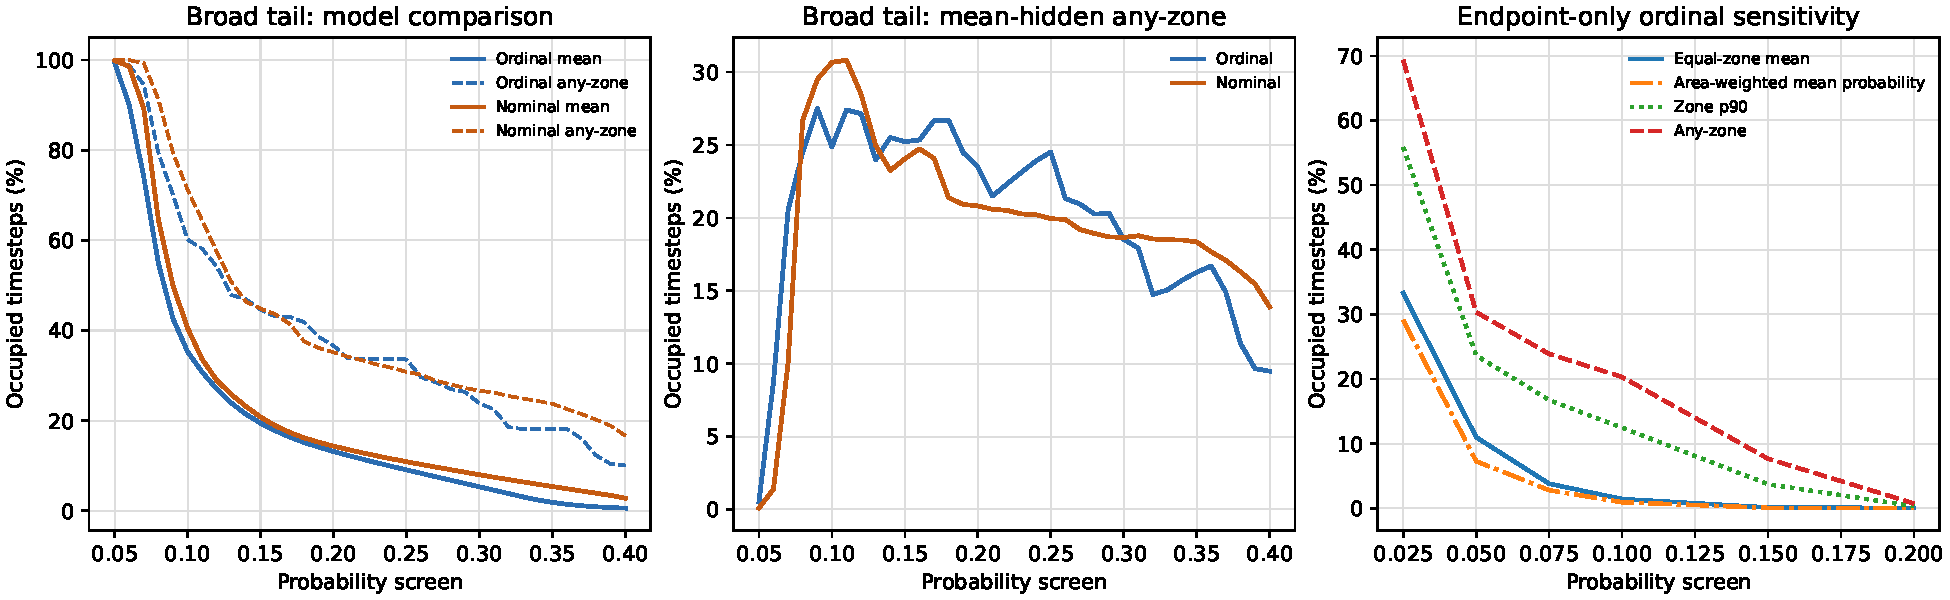
\includegraphics[width=0.66\linewidth]{figs/p_tail_threshold_sensitivity.pdf}
    \caption{Probability-screen and tail-definition sensitivity across the full 144-role fixed-reference panel. Left: mean-zone and any-zone screened shares for the primary ordinal and nominal seven-class predictors. Center: the corresponding mean-hidden any-zone share. Right: mean-zone, area-weighted mean-probability, p90-zone, and any-zone screened shares for the endpoint-only probability $p_{\mathrm{outermost}}=\Pr(\mathrm{TSV}\in\{-3,+3\})$. Absolute shares are model-, threshold-, and event-definition-conditional, while the mean-to-any-zone ordering persists across the tested specifications.}
    \label{fig:tail_threshold_sensitivity}
\end{figure}

Figure~\ref{fig:tail_threshold_sensitivity} tests whether this hidden-zone effect depends on the selected reporting screen, predictor form, or tail definition. For the primary tail, absolute exceedance falls as the screen becomes stricter, but any-zone exceedance remains well above mean-zone exceedance. At $\tau=0.10$, mean-zone exceedance was 35.30\% and any-zone exceedance was 60.18\%; at $\tau=0.30$, they were 5.30\% and 23.83\%, respectively. Hidden any-zone exceedance remained at least 18.5\% from $\tau=0.10$ to 0.30. The nominal predictor preserved the same spatial ordering, although model differences in absolute rates were threshold-dependent and reached 11.05 percentage points for the any-zone statistic at $\tau=0.10$. The no-PMV predictor also showed the same pattern: at $\tau=0.20$, mean-zone exceedance was 13.85\%, any-zone exceedance was 37.52\%, and hidden any-zone exceedance was 23.67\%.

The endpoint-only event provides a stricter category-boundary check. At an endpoint-probability screen of 0.05, mean-zone exceedance was 10.99\%, any-zone exceedance was 30.34\%, and the mean-hidden any-zone share was 19.35\%. Across the prespecified endpoint screens from 0.025 to 0.20, the paired any-zone-minus-mean-zone gap remained positive; its conditional bootstrap range narrowed from 36.03 [34.58, 37.48] percentage points at 0.025 to 0.70 [0.41, 1.04] at 0.20. Because the held-out corpus contains only 1{,}350 endpoint observations among 22{,}223 test records, this result is a support-limited bounding sensitivity, not a replacement outcome.

The area-weighted zone-time diagnostic gives a useful check on this result. Its close agreement with the mean-zone value does not remove the localized high-tail signal. It shows that much of the hidden any-zone exceedance comes from smaller perimeter zones rather than from the largest core zones.

\begin{table}[htbp]
\centering
\caption{Zone aggregation summary by city. Mean, any-zone, and p90-zone columns report modeled high-tail exceedance at $p_{\mathrm{tail}}\ge0.20$. Any-zone exceedance is the share of occupied timesteps for which the maximum zone value satisfies $\max_z p_{\mathrm{tail},z}\ge0.20$. Hidden high-tail exceedance means the mean-zone value is below 0.20 while at least one zone is at or above 0.20.}
\label{tab:zone_aggregation_summary}
\scriptsize
\resizebox{\textwidth}{!}{%
\begin{tabular}{lrrrrr}
\toprule
\textbf{City} & \textbf{Mean-zone (\%)} & \textbf{Area-weighted zone-time (\%)} & \textbf{Any-zone (\%)} & \textbf{p90-zone (\%)} & \textbf{Hidden any-zone (\%)} \\
\midrule
Ahmedabad & 16.65 & 17.21 & 53.88 & 41.63 & 37.22 \\
Beijing & 5.37 & 5.75 & 15.44 & 9.86 & 10.07 \\
Guangzhou & 12.22 & 11.63 & 31.70 & 22.90 & 19.47 \\
Houston & 12.09 & 10.81 & 27.82 & 22.00 & 15.73 \\
Kolkata & 19.53 & 20.36 & 46.80 & 35.92 & 27.26 \\
Phoenix & 13.02 & 11.48 & 44.23 & 34.67 & 31.22 \\
\bottomrule
\end{tabular}
}
\end{table}

The zones with the largest high-tail screened shares were perimeter zones, especially P1, the south perimeter orientation in this DOE Medium Office geometry. The largest high-tail exceedance rates were 30.24\% for \texttt{perimeter\_bot\_zn\_1}, 27.62\% for \texttt{perimeter\_mid\_zn\_1}, and 23.27\% for \texttt{perimeter\_top\_zn\_1}. Each of these zones accounts for about 4.16\% of conditioned floor area, while each core zone accounts for about 19.74\%. Thus, the largest modeled local tail exceedance occurs in relatively small perimeter zones, while the building-level area-weighted signal is shaped strongly by the larger core zones.

Figure~\ref{fig:zone_size_mosaic} shows that this local pattern changes by city and time slice. Beijing remains comparatively low: the largest pooled zone-specific screened share rises from 7.1\% in the reference slice to 14.9\% in the late-2080s slice. Guangzhou shows a clearer future-weather transition, with its largest zone-specific share increasing from 20.2\% in the reference slice to 28.9\% in the mid-2050s and 41.7\% in the late-2080s. Kolkata reaches higher exceedance earlier: its corresponding value is 31.5\% in the reference slice, 48.2\% in the mid-2050s, and 55.4\% in the late-2080s. Ahmedabad has a different structure: south-perimeter P1 already has a high screened share, but non-P1 perimeter and core zones remain much lower until the late-2080s. This is why Ahmedabad can appear high under an any-zone view while the broader zone field is less uniformly elevated than Kolkata.

\begin{figure}[p]
    \centering
    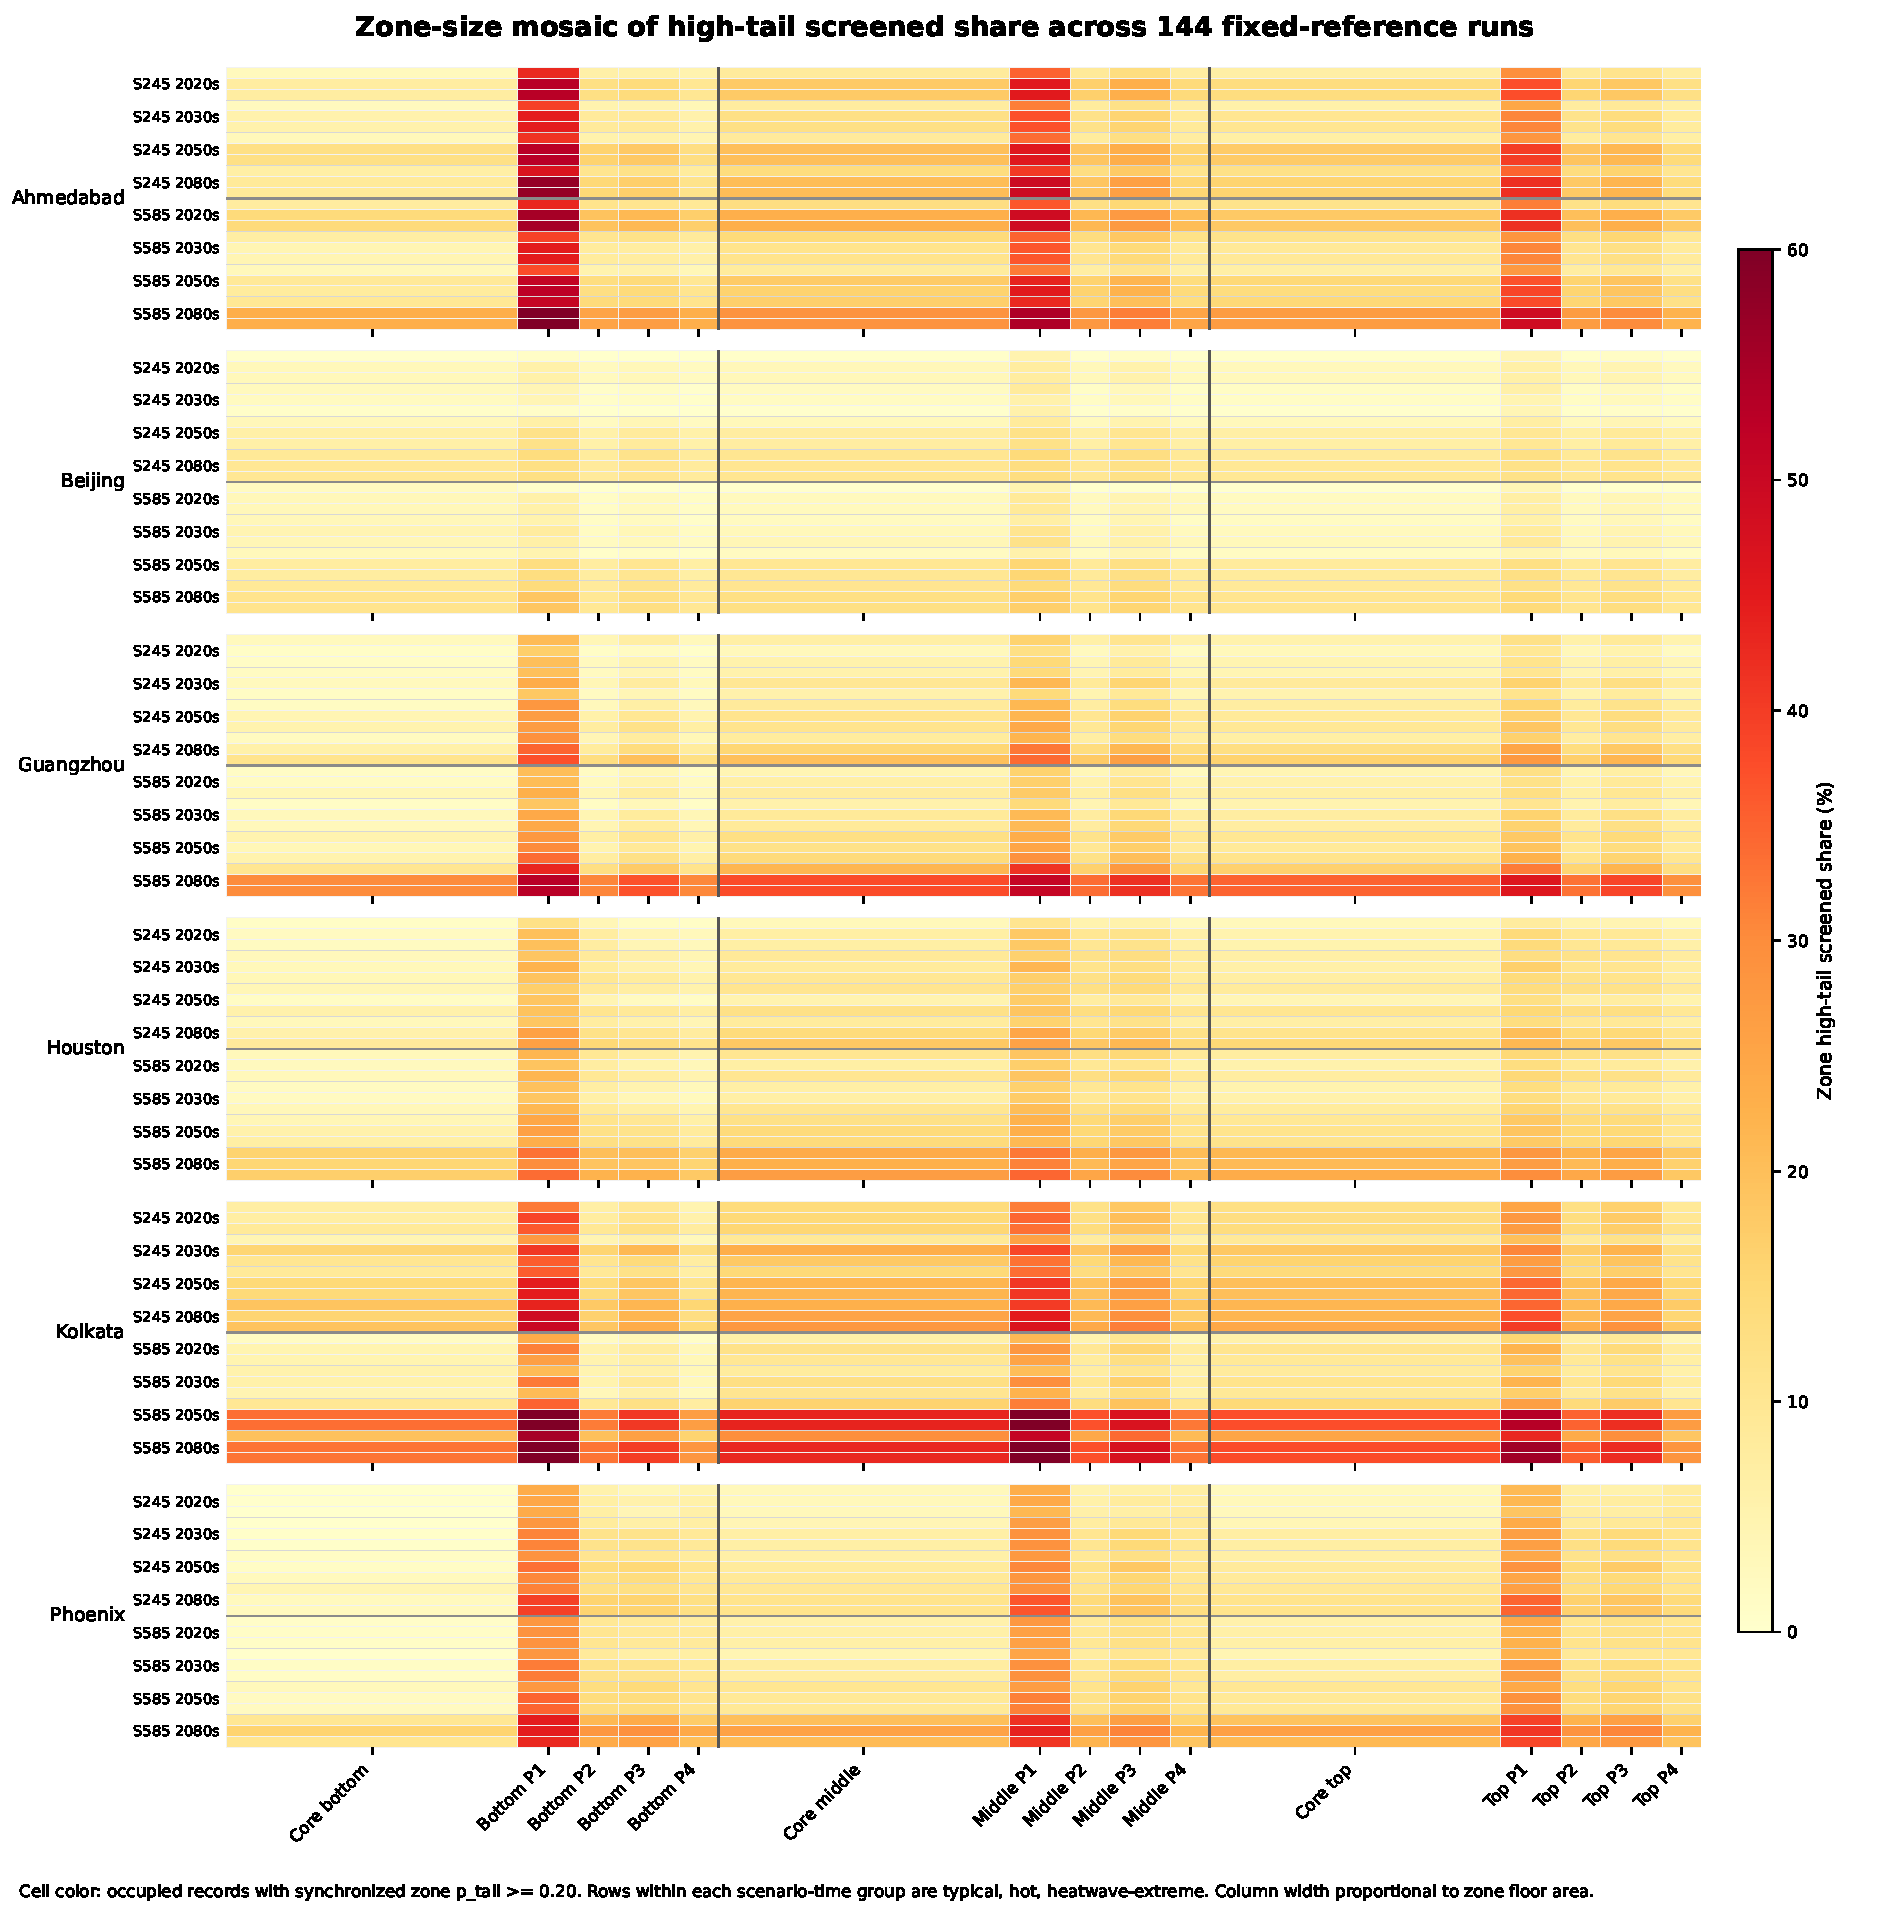
\includegraphics[width=\linewidth,height=0.86\textheight,keepaspectratio]{figs/zone_size_mosaic_heatmap_area.pdf}
    \caption{Zone-size mosaic of modeled high-tail exceedance across the 144-case fixed-reference panel. Cell color reports the share of occupied records in each case-zone pair with $p_{\mathrm{tail}}\ge0.20$. Column width is proportional to conditioned floor area, so the figure compares local tail exceedance with the physical size of the zone carrying that signal. Core bottom, core middle, and core top are the three core zones of the DOE Medium Office prototype; Bottom P1--P4, Middle P1--P4, and Top P1--P4 are the four perimeter zones on each floor level. P1--P4 denote perimeter orientations: P1 south, P2 east, P3 north, and P4 west. The conditioned top zones sit below the top-floor plenum and roof assembly, so ``top'' should not be read as a directly roof-exposed room condition. Rows within each scenario-time group are ordered as typical, hot, and heatwave-extreme weather files.}
    \label{fig:zone_size_mosaic}
\end{figure}

Figure~\ref{fig:zone_floor_position} was generated as a direct check on the floor/orientation reading from Fig.~\ref{fig:zone_size_mosaic}. It prevents over-reading the mosaic as a simple floor-height effect. Area-weighted high-tail exceedance was 10.79\% for the bottom floor, 14.79\% for the middle floor, and 13.03\% for the top floor. The middle floor had the highest area-weighted floor exceedance in 135 of 144 cases. Bottom-floor exceedance was highest only under an any-zone-within-floor summary, where the south perimeter zone P1 dominated. Bottom P1 had 30.24\% high-tail exceedance, compared with 27.62\% for middle P1 and 23.27\% for top P1. For the other perimeter orientations, bottom was not the highest. We therefore interpret the floor pattern as a prototype-specific interaction between perimeter orientation, floor construction, and zone conditioning, not as a general result that lower floors have higher screened shares than upper floors. High-tail states were warm-dominant in all zones under the $p_{\mathrm{tail}}\ge0.20$ screen.

\begin{figure}[htbp]
    \centering
    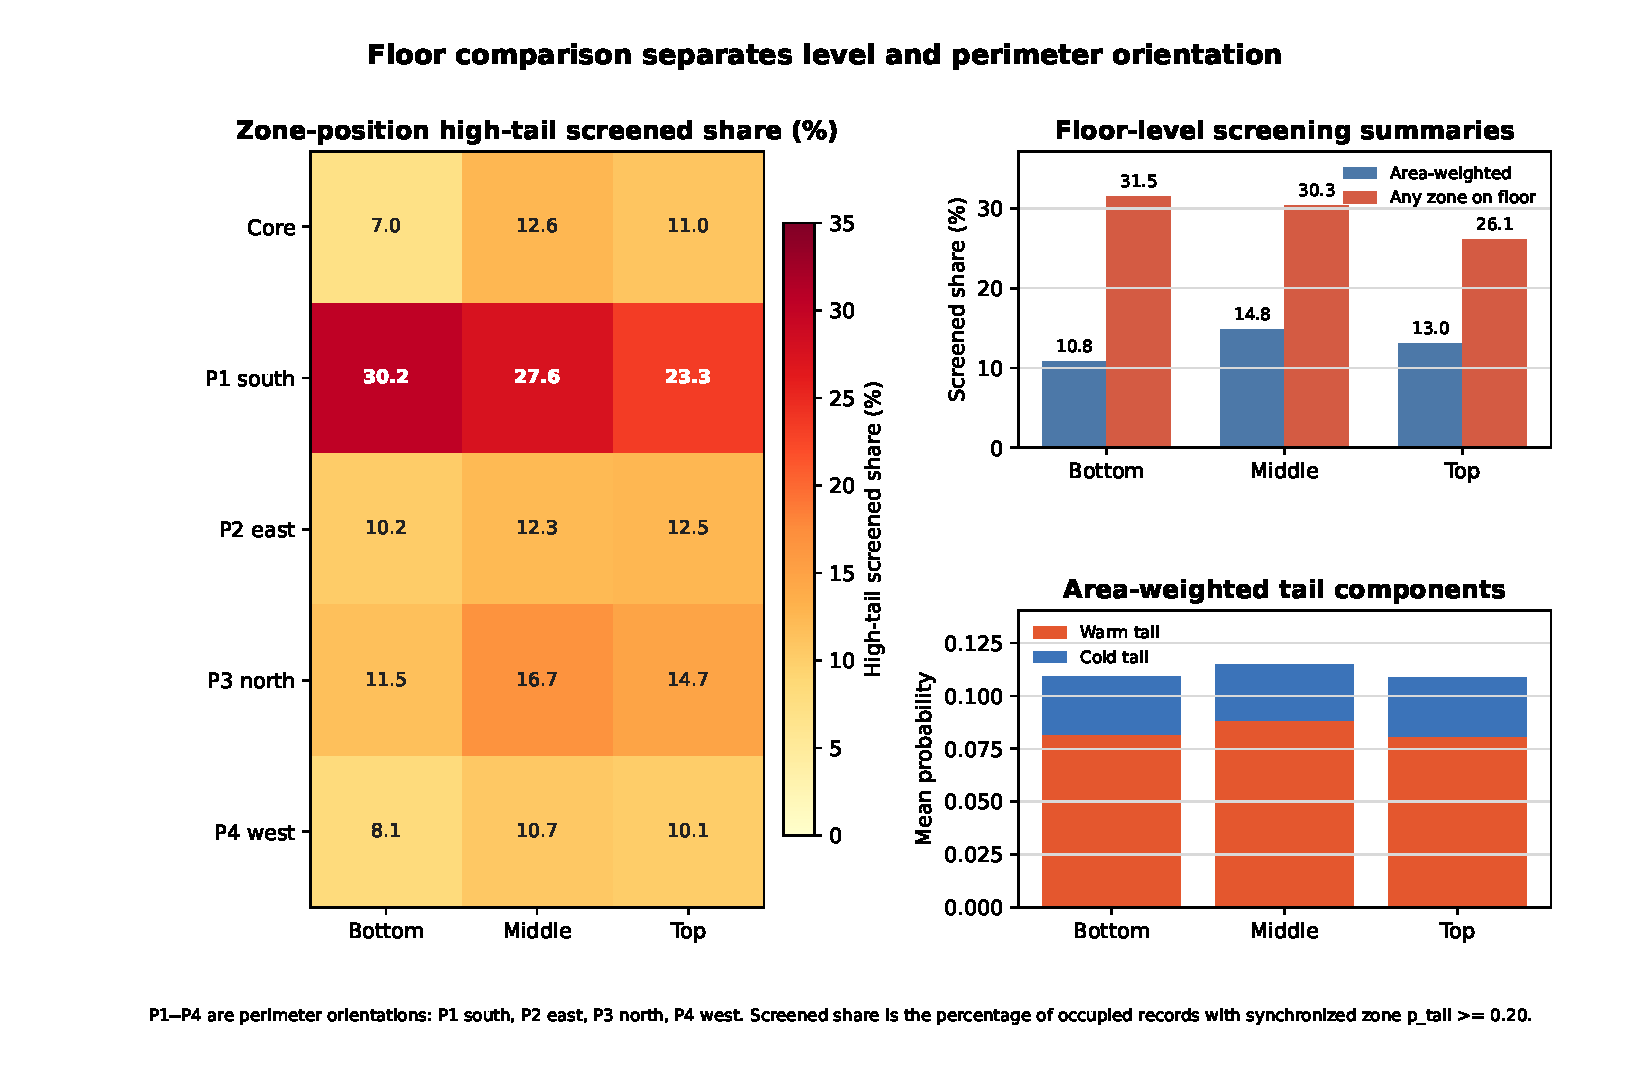
\includegraphics[width=\linewidth]{figs/zone_floor_position_comparison.pdf}
    \caption{Floor-position comparison for the 144-case fixed-reference panel. The heat map reports modeled high-tail exceedance by floor and zone position. P1--P4 are the perimeter orientations in the DOE Medium Office prototype: P1 south, P2 east, P3 north, and P4 west. Area-weighted floor exceedance summarizes zone-time records using conditioned floor area, while any-zone floor exceedance reports the share of occupied records in which at least one zone on that floor exceeds $p_{\mathrm{tail}}\ge0.20$. Tail-component bars show that floor differences are driven mainly by the warm tail.}
    \label{fig:zone_floor_position}
\end{figure}

\subsection{Weather-to-zone association audit}

The recorded states support a mechanism-consistent three-link interpretation, although not causal decomposition. Across the 144 role-labelled cases, the median within-case Spearman association between outdoor dry-bulb temperature and mean-zone operative temperature was 0.824 (interquartile range 0.753--0.897). The median association between operative temperature and $p_{\mathrm{tail}}$ was 0.855 (0.794--0.917), while the descriptive association between requested zone cooling rate and $p_{\mathrm{tail}}$ was 0.574 (0.411--0.629). The cooling association indicates coincident HVAC response; without unmet-load or component-capacity outputs it does not establish plant saturation.

Matched baseline-to-late comparisons make the pathway clearer. Annual mean outdoor temperature, occupied mean-zone operative temperature, mean $p_{\mathrm{tail}}$, and mean-zone screened share all increased in 36 of 36 city--scenario--selection-role comparisons. The median changes were $+2.13$\,\degree C outdoors, $+0.50$\,\degree C operative, $+0.0259$ in mean $p_{\mathrm{tail}}$, and $+10.13$ percentage points in screened share. After duplicate roles were collapsed, screened share increased from 0.19\% in the 20--25\,\degree C outdoor-temperature stratum to 52.69\% at outdoor temperatures of at least 35\,\degree C. Across the same 119 unique states, the three south-perimeter zones averaged 25.93\% high-tail exceedance, compared with 11.21\% for the other nine perimeter zones.

Whole-year correlations should not be read as temperature-response coefficients. Ten of 144 annual operative-temperature--total-tail correlations were negative, all in Beijing, because whole-year season mixing interacts with the predictor's running-mean outdoor context and other covariates. Under outdoor temperature at or above 25\,\degree C, however, the operative-temperature--warm-tail association was positive in every case, with median $\rho=0.977$. The combined evidence is therefore consistent with hotter selected weather shifting simulated operative conditions and warm-tail probability while the fixed HVAC system responds. It does not isolate facade solar gain, humidity, envelope heat flux, or equipment capacity as independent causes.

\subsection{Metabolic-input sensitivity}

The metabolic-input sensitivity shows that representative occupant assumptions can materially change the TSV-tail profile even when the simulated thermal environments are held fixed. Table~\ref{tab:metabolic_scenario_summary} is a panel-level summary across both SSP pathways, all six cities, four time slices, and three annual weather severities; it is not a pathway-specific estimate. Across 216{,}483{,}840 zone-profile probability evaluations, the mean spread in mean-zone $p_{\mathrm{tail}}$ across the six metabolic profiles was 0.074, with a 95th percentile spread of 0.209. For max-zone $p_{\mathrm{tail}}$, the mean spread was 0.137 and the 95th percentile spread was 0.327.

Changing the metabolic profile also changed threshold status. Mean-zone high-tail status flipped across metabolic profiles in 18.99\% of occupied records, and max-zone high-tail status flipped in 38.66\%. When the S-real profile remained below the high-tail cutoff, some other metabolic profile crossed it in 18.80\% of mean-zone records and 36.51\% of any-zone records. Because the fixed-reference panel is warm-tail dominated, lower metabolic-load profiles generally reduced the predicted high-tail screened share. In this diagnostic, a lower metabolic input means the same simulated thermal environment is interpreted by the reported-TSV model with less occupant metabolic heat.

\begin{table}[htbp]
\centering
\caption{Panel-level metabolic-spread results across the full 144-case fixed-reference panel: six cities, SSP2-4.5 and SSP5-8.5, four time slices, and three annual weather severities. Values are pooled across pathways and recomputed over fixed environmental traces; EnergyPlus was not rerun with altered occupant heat gains.}
\label{tab:metabolic_scenario_summary}
\footnotesize
\begin{tabular}{lrrrr}
\toprule
\textbf{Profile} & \textbf{W/person} & \textbf{met} & \textbf{Mean-zone high-tail (\%)} & \textbf{Any-zone high-tail (\%)} \\
\midrule
COMP-Lo & 90.0 & 0.900 & 3.32 & 13.82 \\
S-real & 93.2 & 0.932 & 3.10 & 14.89 \\
COMP-Med & 100.0 & 1.000 & 7.97 & 29.78 \\
EQ-Max & 108.0 & 1.080 & 21.20 & 45.37 \\
COMP-Hi & 110.0 & 1.100 & 13.66 & 38.44 \\
LEGACY & 120.0 & 1.200 & 17.32 & 47.87 \\
\bottomrule
\end{tabular}
\end{table}

The response is not strictly monotone across all adjacent profiles; in particular, the calibrated model gives a lower mean-zone high-tail screened share at 110 W/person than at 108 W/person. We therefore interpret this section as a sensitivity diagnostic across metabolic assumptions, not as a smooth physiological dose-response curve. The practical result is still clear: the single representative occupant assumption can hide a substantial range of predicted reported-TSV tail screening.

The zone-resolved profile summaries show where this sensitivity is concentrated. Across the 2{,}160 case-zone summaries for each profile, the mean case-zone high-tail screened share was 3.27\% for COMP-Lo, 3.26\% for S-real, 8.65\% for COMP-Med, 19.25\% for EQ-Max, 15.37\% for COMP-Hi, and 18.77\% for LEGACY. The spread in case-zone screened share across the six profiles averaged 16.85 percentage points, with a 95th percentile of 36.15 percentage points. The largest mean spreads occurred in the south perimeter zones: Bottom P1 (30.44 percentage points), Middle P1 (28.64 percentage points), and Top P1 (24.96 percentage points). This reinforces the diagnostic claim: metabolic assumptions and zone aggregation interact, so a single representative occupant can hide spatially localized profile sensitivity.

\begin{figure}[htbp]
    \centering
    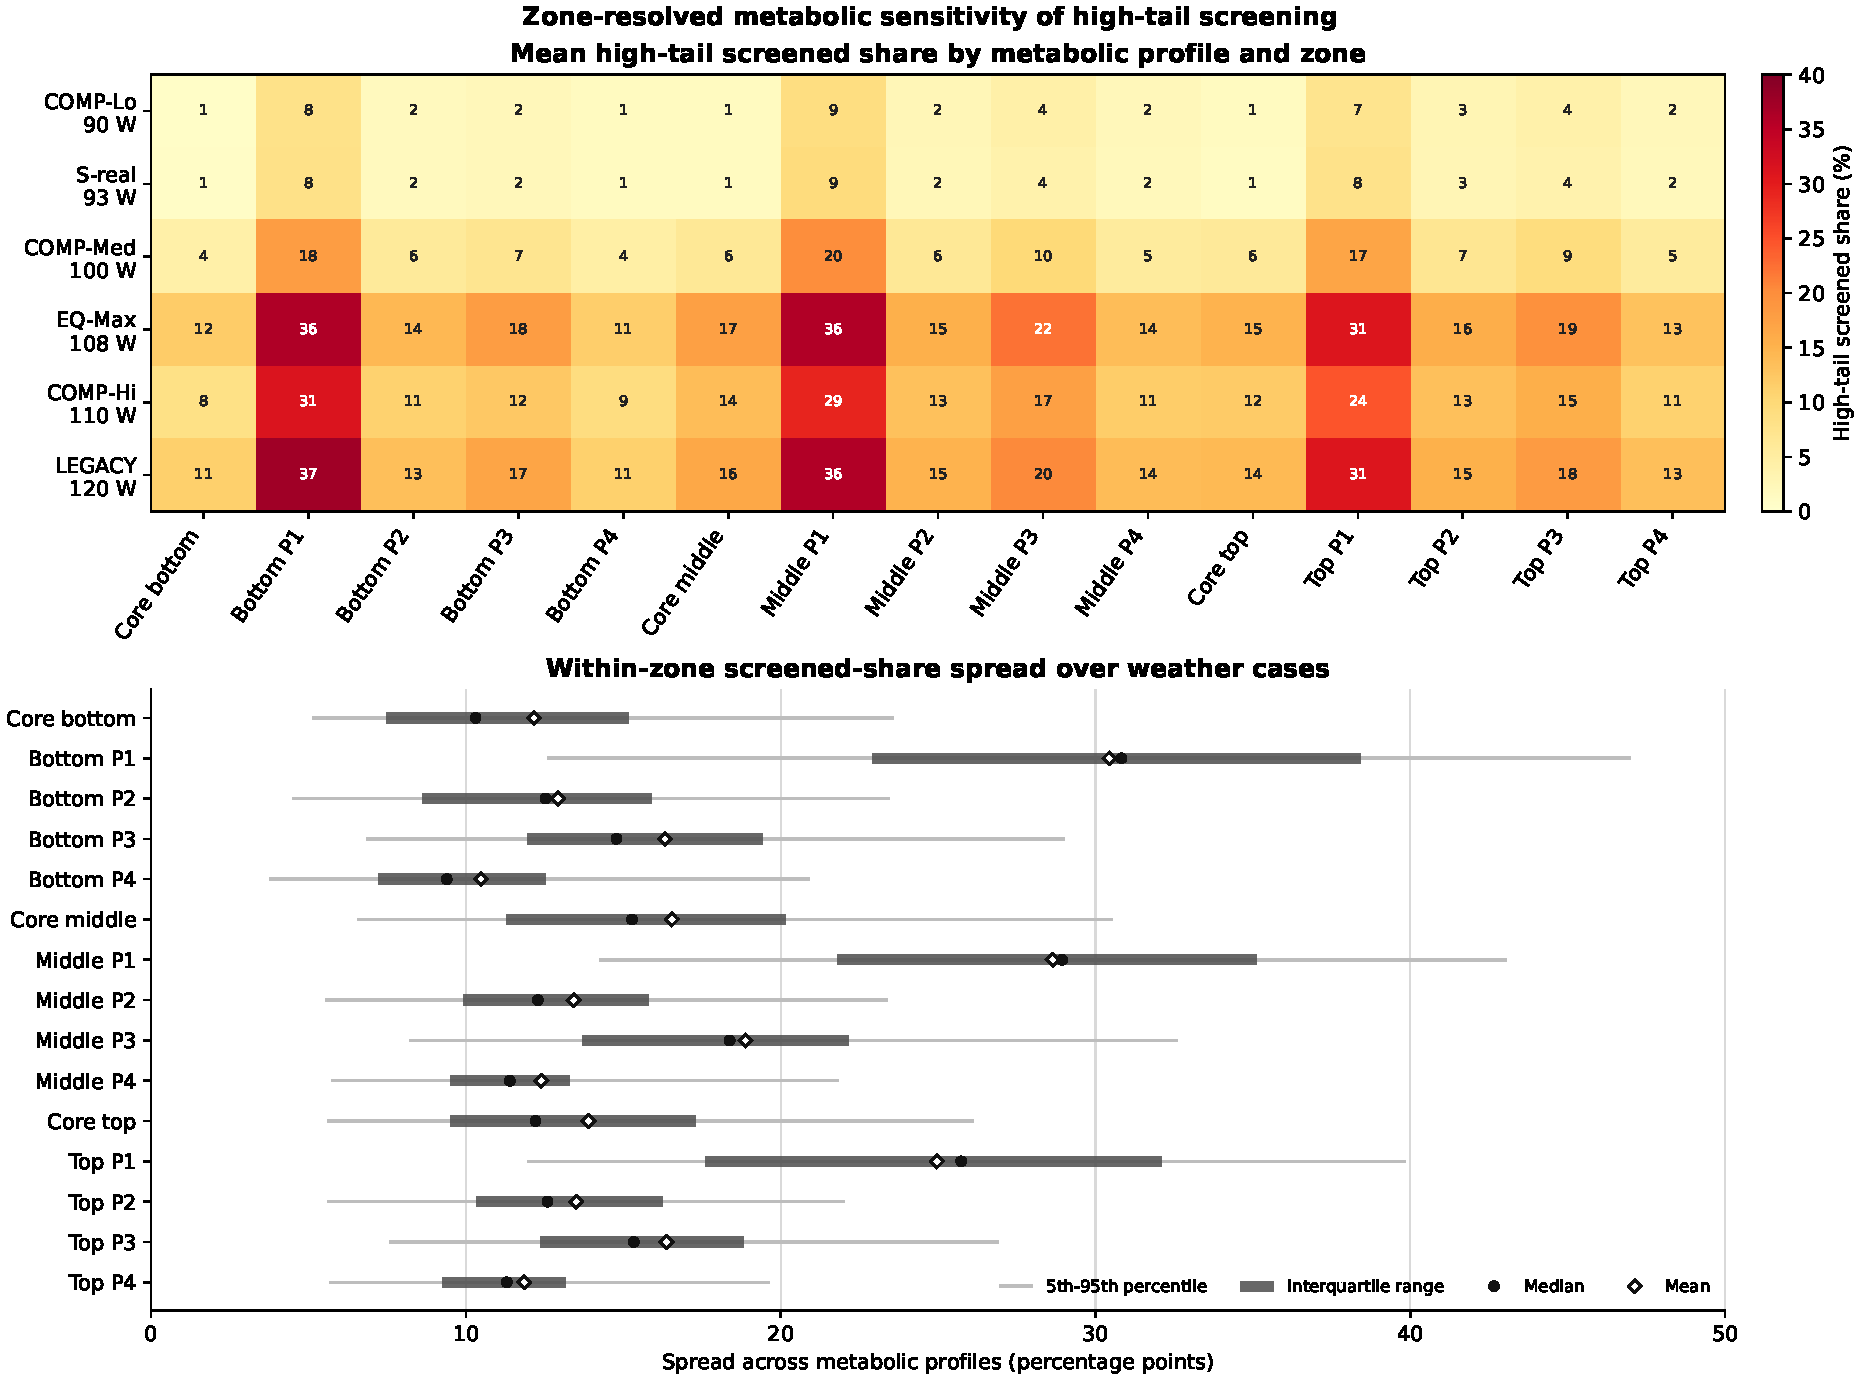
\includegraphics[width=\linewidth]{figs/zone_metabolic_profile_summary.pdf}
    \caption{Zone-resolved metabolic sensitivity of high-tail screening. Top: mean case-zone screened share by metabolic profile and zone. Bottom: within-zone spread across metabolic profiles summarized over the 144 weather cases. Points mark medians, diamonds mark means, thick intervals show the interquartile range, and thin intervals show the 5th--95th percentile range. Values are recomputed over fixed simulated environments, so the differences reflect representation sensitivity to metabolic inputs rather than altered internal heat gains or measured occupant exposure.}
    \label{fig:metabolic_profile_summary}
\end{figure}
